\begin{algorithm}[t]
\caption{Safe Flow Expansion}
\label{alg:sfe}
\small
\DontPrintSemicolon

\KwIn{pretrained CFM $\theta_0$; verifier $v_\gamma$;
      dynamics $f$; execution cost $C$, rounds $N$; parallel episodes $P$;
      proposal and verification budgets $K\ge B$}
\KwOut{expanded CFM $\theta_N$}
$\mathcal B_0, \mathcal D_0 \gets\varnothing$\;
\For{$n\gets0$ \KwTo $N-1$}{
    $\sigma_n\gets
    \textsc{UpdateUncertainty}(\mathcal B_n)$\;

    \Repeat{$|\{\boldsymbol{\tau}\in\mathcal R_n: \textsc{Success}(\boldsymbol{\tau})\}|\ge P$}{
        $\mathcal R_n\gets P$ parallel rollouts under $\theta_n$\;

        \ForEach{replanning step $k$ in the active rollouts}{
            Context $\o_k=(\mathbf o_k,\gamma_k)$\;

            Draw $B$ candidates from $K$ proposals:
            \[
            \hat{\mathbf u}^{(1:B)}
            \sim
            p_1^{\theta_n}
            (\hat{\mathbf u}\mid\o_k)
            \exp\!\left(
            \sigma_n(\phi_s(\hat{\mathbf u}))/ \beta
            \right)/Z
            \]

            Verify $y_j\gets
            v_{\gamma_k}
            (\o_k,\hat{\mathbf u}^{(j)})$,
            \quad $j=1,\ldots,B$:
            \[
            \mathcal J_k^+\gets
            \left\{
            j\in\{1,\ldots,B\}:y_j=1
            \right\}
            \]
            
            \If{$\mathcal J_k^+=\varnothing$}{
                \textsc{RestartRollout}()
            }
            
            $j^\star\gets
            \displaystyle
            \arg\min_{j\in\mathcal J_k^+}
            C(\o_k,\hat{\mathbf u}^{(j)})$\;

            Rollout 
            $\mathbf u_k\gets
            [\hat{\mathbf u}^{(j^\star)}]_0,
            \;
            \mathbf x_{k+1}\gets
            f(\mathbf x_k,\mathbf u_k)$
            % \tcp*[h]{rollout}
        }

        $\mathcal D_n\gets
        \mathcal D_n\cup
        \{(\o_k, \gamma_k, \hat{u}^{(j)}, y_j)
        \}_{j=1}^B$\;
    }
    $\mathcal B_{n+1}\gets
    \textsc{UpdateBuffer}(\mathcal B_n,\mathcal D_n)$\;

    $\theta_{n+1}\gets
    \textsc{UpdateCFM}(\theta_n,\mathcal D_n)$\;
}
\Return{$\theta_N$}\;
\end{algorithm}

\section{Appendix: Safe Flow Expansion Analysis}\label{sec:safe-flow-expansion-analysis}

% NOTE (blue edits): the statistical model now precedes the reachability analysis, so the
% reachable operator is defined once, after the objects it depends on. This removes the
% duplicate \label{eq:reachable-action-set} and the forward references.

\noindent\textbf{Verifier uncertainty model.}
We use bandits with preference feedback theory to provide confidence intervals for verifier uncertainty. Fix the context and safety pair \((\xi,\gamma)\), then the noised flow representation induces the conditional representation space
\begin{equation}
    \begin{aligned}
        \phi_s(\cdot;\xi,\gamma)&:\mathcal U^H\rightarrow
        \mathcal Z_{\xi,\gamma},\\
        \mathcal Z_{\xi,\gamma}
        &:=
        \left\{
        \phi_s(\hat{\mathbf u};\xi,\gamma):
        \hat{\mathbf u}\in\mathcal U^H
        \right\}.
    \end{aligned}
    \label{eq:conditional-representation-space}
\end{equation}
For \(z=\phi_s(\hat{\mathbf u};\xi,\gamma)\), the binary verifier feedback can be modeled as the composition of sigmoid function and unknown validity function on the representation space
\begin{equation}
    \Pr(y=1\mid z)=s(g(z)), \quad
    s(a):=(1+\exp(-a))^{-1},
    \label{eq:logistic-verifier-model}
\end{equation}
where $h>0$ is a threshold, \(g\in\mathcal H_k\) is an unknown function in the Reproducing Kernel Hilbert Space (RKHS) associated
with kernel \(k\), with \(\|g\|_k\le B\). Then the valid representation set is
\begin{equation}
\Omega_* := \{z\in Z : s(g(z)) \ge h\}.
\label{eq:prob_valid_set}
\end{equation}
Let \(\mu_t\) denote the
regularized kernel logistic estimator obtained from \(t\) verified
queries \(\{(z_i,y_i)\}_{i=1}^t\) (See Prop.1~\cite{pasztor2024bandits}). Its uncertainty score is
\begin{equation}
    \sigma_t^2(z)
    :=
    k(z,z)
    -
    k_t(z)^\top
    \left(K_t+\lambda\kappa I_t\right)^{-1}
    k_t(z),
    \label{eq:kernel-logistic-uncertainty}
\end{equation}
where \([k_t(z)]_i=k(z_i,z)\), \([K_t]_{ij}=k(z_i,z_j)\),
\(\lambda>0\), and
\(\kappa:=\sup_{|a|\le B}1/\dot{s}(a)\).
\begin{lemma}[Thm.2~\cite{pasztor2024bandits}]
\label{thm:kernelized-logistic-confidence}
Let
\(A\subseteq\mathcal Z_{\xi,\gamma}\) be compact and suppose
\(k(z,z)\le1\) for all \(z\in A\). Assume
\(g\in\mathcal H_k\) and \(\|g\|_k\le B\). For \(0<\delta<1\), define the interval and information gain:
\begin{align}
    \beta_t^A(\delta)
    &:=
    4L_sB+
    2L_s
    \sqrt{
    \frac{2\kappa}{\lambda}
    \left(\mathcal I_t^A+\log(1/\delta)\right)
    },
    \label{eq:logistic-confidence-radius}\\
    \mathcal I_t^A
    &:=
    \max_{z_1,\ldots,z_t\in A}
    \frac{1}{2}
    \log\det\left(
    I_t+(\lambda\kappa)^{-1}K_t
    \right),
    \label{eq:maximum-information-gain}
\end{align}
where \(L_s:=\sup_{|a|\le B}\dot{s}(a)\). Then
\begin{equation}
    \begin{aligned}
        \Pr\bigl(\forall t\ge1,\ \forall z\in A:\\
        \left|s(\mu_t(z))-s(g(z))\right|
        &\le\beta_t^A(\delta)\sigma_t(z)
        \bigr)
        \ge1-\delta.
    \end{aligned}
    \label{eq:anytime-logistic-confidence}
\end{equation}
\end{lemma}
Thus a single event of probability at least \(1-\delta\) controls all
query rounds at time $t$ and representation features $z$. In particular, the lower
confidence bound
\(
s(\mu_t(z))-\beta_t^A(\delta)\sigma_t(z)
\)
is used below to expand the verifier-certified set. We want to pullback to our original action space~\footnote{The canonical kernel metric is used $d_k(z,z')
:=
\left\|
k(z,\cdot)-k(z',\cdot)
\right\|_{\mathcal H_k}$}., define
\begin{equation}
d_{\phi,k}^{\xi,\gamma}
(\hat{\mathbf u},\hat{\mathbf u}')
:=
d_k\!\left(
\phi_s(\hat{\mathbf u};\xi,\gamma),
\phi_s(\hat{\mathbf u}';\xi,\gamma)
\right).
\label{eq:pullback-kernel-metric}
\end{equation}
By the reproducing property in RKHS, under the assumption that $s$ is $L_s$--Lipschitz,
\begin{equation}
\left|
\rho_\gamma(\hat{\mathbf u})
-\rho_\gamma(\hat{\mathbf u}')
\right|
\le
L_sB\,
d_{\phi,k}^{\xi,\gamma}
(\hat{\mathbf u},\hat{\mathbf u}').
\label{eq:rkhs-spatial-bound}
\end{equation}

We can now define the verifier-certified set from its representation surrogate~\eqref{eq:logistic-verifier-model}
\begin{equation}
\mathcal V_{\gamma}(\xi)
:=
\left\{
\hat{\mathbf u}\in\mathcal U^H:
\rho_\gamma(\hat{\mathbf u})\ge h
\right\}.
\label{eq:representation-valid-certified-set}
\end{equation}
The certified generable set is
\begin{equation}
\mathcal G_{\theta_t}^{\tau}(\xi,\gamma)
:=
\Omega_{\theta_t}^{\tau}(\xi,\gamma)
\cap
\mathcal V_\gamma(\xi).
\label{eq:certified-generable-set}
\end{equation}

\noindent\textbf{Reachability analysis.}
Given the statistical model in~\eqref{eq:prob_valid_set}, binary feedback in the original action space $\mathcal U^H$ is given as \( \rho_\gamma(\hat{\mathbf u})=s\!\left(g(\phi_s(\hat{\mathbf u};\xi,\gamma))\right)\).
Let \(S_t\) denote the action set certified by the lower confidence
bound after \(t\) verified queries, and let
\(\varnothing\neq S_0\subseteq
\mathcal G_{\theta_0}^{\tau}(\xi,\gamma)\) denote an initially
generable valid seed. For \(\epsilon>0\) and the fixed pair
\((\xi,\gamma)\), define the one-step reachable operator as:
\begin{equation}
\begin{aligned}
R_\epsilon(S)
&:=
\Bigl\{
\hat{\mathbf u}\in\mathcal U^H:
\exists\hat{\mathbf u}'\in S\ \text{s.t.}\\[-1mm]
&\quad
\rho_\gamma(\hat{\mathbf u}')-\epsilon
-L_sB\,d_{\phi,k}^{\xi,\gamma}
(\hat{\mathbf u},\hat{\mathbf u}')\ge h
\Bigr\}.
\end{aligned}
\label{eq:reachable-action-set}
\end{equation}
Subsequently, we can define
\begin{equation}
\begin{aligned}
R_\epsilon^0(S)&:=S,\qquad
R_\epsilon^{j+1}(S):=R_\epsilon(R_\epsilon^j(S)),\\
R_\epsilon^{\le r}(S)&:=
\bigcup_{j=0}^{r}R_\epsilon^j(S).
\end{aligned}
\label{eq:cumulative-reachable-action-set}
\end{equation}

{\color{blue}
The seed is supplied by the planner rather than assumed: by Proposition~\ref{prop: 3} every action window accepted by MPPI-DCBF is verifier-positive, so $S_0\neq\varnothing$ whenever the demonstrations are non-empty. The analysis needs the mildly stronger statement that it occupies volume.
\begin{assumption}[Positive-volume certified seed]
\label{ass:positive-volume-seed}
For the fixed pair $(\xi,\gamma)$, the initial certified seed satisfies
$S_0\subseteq\mathcal G_{\theta_0}^{\tau}(\xi,\gamma)$ and
$\operatorname{Vol}(S_0)>0$.
\end{assumption}
}

\begin{lemma}[Corollary~4.2~\cite{de2026active}]
\label{lem:reachable-generable-coverage}
The following is its conditional action-space adaptation. Fix \(r\ge1\)
and let \(T^\star=rT\) be verifier queries. Under the
assumptions in Appendix~\ref{sec:safe-flow-expansion-analysis}, with probability at least \(1-\delta\),
\begin{equation}
R_\epsilon^r(S_0)
\subseteq
R_\epsilon^{\le r}(S_0)
\subseteq
S_{T^\star}
\subseteq
\Omega_{\theta_{T^\star}}^\tau(\xi,\gamma).
\label{eq:main_inclusion}
\end{equation}
\end{lemma}

Define the coverage event and its deterministic verifier-safe part as
\begin{align}
\mathcal E_{\mathrm{cov}}
&:=
\left\{
R_\epsilon^{\le r}(S_0)
\subseteq S_{T^\star}
\subseteq\Omega_{\theta_{T^\star}}^\tau(\xi,\gamma)
\right\},
\label{eq:coverage-event}\\
A_{\gamma,r}(\xi)
&:=
R_\epsilon^{\le r}(S_0)
\cap\Omega^\star(\xi,\gamma).
\label{eq:safe-reachable-region}
\end{align}
On \(\mathcal E_{\mathrm{cov}}\),
\begin{equation}
A_{\gamma,r}(\xi)
\subseteq
\Omega_{\theta_{T^\star}}^\tau(\xi,\gamma)
\cap\Omega^\star(\xi,\gamma).
\label{eq:safe-generable-inclusion}
\end{equation}
Moreover, Assumption~\ref{ass:positive-volume-seed} gives
\begin{equation}
\begin{aligned}
m_\gamma(\xi)
&:=
\operatorname{Vol}\!\left(A_{\gamma,r}(\xi)\right)\\
&\ge\operatorname{Vol}(S_0)>0.
\end{aligned}
\label{eq:positive-reachable-volume}
\end{equation}

Having defined the conditional generable set~\eqref{eq:conditional-generable-set} and the verifier-valid action set~\eqref{eq:representation-valid-certified-set}, and the rechable operator~\eqref{eq:reachable-action-set}, we now state the main theorem on how set coverage via the expansion mechanism translates into the probability of obtaining a safe action window under a finite parallel sampling budget. The result separates the high-probability coverage guarantee over the expansion process from the deployment-time probability induced by sampling the learned policy.

\begin{theorem}[Availability of a multi-step safe action]
\label{thm:safe-action-availability}
Assume the conditions of Lemma~\ref{lem:reachable-generable-coverage} and Lemma~\ref{thm:kernelized-logistic-confidence}, with $m_\gamma(\xi):=\operatorname{Vol}\!\left(R_\epsilon^r(S_0)\cap\Omega^\star(\xi,\gamma)\right)>0.$
After the safe flow expansion in
Lemma~\ref{lem:reachable-generable-coverage}, draw \(K\)
conditionally independent samples $\hat{\mathbf u}^{(1:K)}
\overset{\mathrm{i.i.d.}}{\sim}p_1^{\theta_{\hat n}}(\cdot\mid\xi,\gamma)$. Then conditioned on the \(1-\delta\) coverage event in Lemma~\ref{lem:reachable-generable-coverage},
\begin{align}
&\Pr\!\left(
\exists j\le K:
v_\gamma(\hat{\mathbf u}^{(j)};\xi)=1
\right)\\
&\ge
1-
\left(1-\tau m_\gamma(\xi)\right)^K
\ge
1-\exp\!\left(-K\tau m_\gamma(\xi)\right).
\label{eq:safe-action-hit-probability}
\end{align}
Consequently, over both expansion and generation randomness the probability of coverage holds and at least one action being safe is $(1-\delta)\left[1-\left(1-\tau m_\gamma(\xi)\right)^K\right].$
\end{theorem}
{\color{red} MH Question 1: If the verifier is not used at deployment, the selected sample could still be unsafe, right?}

{\color{red} MH Q2: this theorem is written for fixed context $\xi$, which may never repeat during the mission}

\begin{proof}
On the coverage event~\eqref{eq:coverage-event}, it holds that $
R_\epsilon^r(S_0)
\subseteq
\Omega_{\theta_{\hat n}}^\tau(\xi,\gamma).
$
Since the probability density lower bound $\tau$ applies to the entire volume $m_\gamma(\xi)$ under the coverage event, hence
\[
\Pr\!\left(
\hat{\mathbf u}\in
R_\epsilon^r(S_0)\cap\Omega^\star(\xi,\gamma)
\right)
\ge
\tau m_\gamma(\xi).
\]
Conditional independence gives the complement probability in
\eqref{eq:safe-action-hit-probability}. Every sample in
\(\Omega^\star(\xi,\gamma)\) passes the deterministic SOCP verifier
and is therefore multi-step safe.
\end{proof}
\begin{corollary}
    Given the same $\xi$, the probability bound~\eqref{eq:safe-action-hit-probability} given by the valid action set $\Omega^\star(\xi,\gamma)$ is monotonically {\color{blue} increasing in the sampling budget $K$ and in the reachable safe volume $m_\gamma(\xi)$, so both a larger parallel budget and a further expansion round can only improve it.}
\end{corollary}

% When the pre-trained policy represents only a few dominant modes, its
% generable set may cover only a small portion of the certified set,
% \begin{equation}
%     \operatorname{Vol}\!\left(
%     \Omega_{\theta_0}^{\tau}(\xi,\gamma)
%     \right)
%     \ll
%     \operatorname{Vol}\!\left(\Omega^\star(\xi,\gamma)\right).
% \end{equation}

% For a fixed target context, the verifier-positive support gap targeted
% by expansion is therefore
% \[
% \Omega^\star(\xi,\gamma)
% \setminus
% \Omega^\tau_{\theta_0}(\xi,\gamma).
% \]
% The valid OOD region targeted by expansion is therefore
% \[
%     \Omega^\star(\xi,\gamma)
%     \setminus
%     \Omega_{\theta_0}^{\tau}(\xi,\gamma).
% \]

% Concretely, for a given context $(\mathbf o,\gamma)$, the pre-trained policy $p_1^{\theta_{\mathrm{0}}}(\cdot\mid\mathbf
% o,\gamma)$  samples only its \emph{generable set}:
% \begin{equation}
% \Omega^{\tau}_{\theta_{\mathrm{0}}}
% (\mathbf o,\gamma)=\{\hat{\mathbf u}: p_1^{\theta_{\mathrm{0}}}(\hat{\mathbf u}\mid\mathbf
% o,\gamma)\ge\tau\},
% \end{equation}
% which is the region likely to be sampled and preferably draws from dominant modes. Here, we abbreviate and refer to the sample as $H$ steps of predicted actions $\mathbf{\hat u}_{k:k+H-1}$ as $\mathbf{\hat u}$. 

% Let $\Omega^{*}(\mathbf o,\gamma)=\{\hat{\mathbf u}: v(\hat{\mathbf u};\mathbf o,\gamma)=1\}$
% denote the \emph{valid action set} certified by the verifier polytope of~\eqref{eq:socp}. Since the planner explores few dominant modes due to \textit{local infeasibility}, it is followed that $\mathrm{Vol}(\Omega^{\tau}_{\theta_0})
% \ll\mathrm{Vol}(\Omega^{*})$. Valid samples will lie in the valid out-of-distribution region $\Omega^{*}\setminus\Omega^{\tau}_
% {\theta_{0}}$. 

% % Here we introduce our flow expansion mechanism, contingent to \cite{de2026active}. For the sake of simplicity, we refer to the sample as $H$ steps of predicted actions ($\mathbf{\hat u}_{k:k+H-1}$). We self-generate the action prediction at each time step and execute predicted actions. This yields trajectory generation, and for those that complete the task (\textit{i.e.,} reach the goal while maintained safe) each action prediction assigned a binary function value of $v(\mathbf{\hat u}_{k:k+H-1})$ viz \eqref{eq:verifier}. 


Fix $(\xi,\gamma)$ and let $\hat{\mathbf u}_0\in
\operatorname{int}(\mathcal U^H)$ be an feasible MPPI--DCBF action. Suppose its rollout satisfies the nominal-polytope inequalities~\ref{eq:nominalpolytope} with strict inequality, $p_1^{\theta_0}(\cdot\mid\xi,\gamma)$ are continuous, and $p_1^{\theta_0}(\hat{\mathbf u}_0\mid\xi,\gamma)>\tau$. Under the conditions of Proposition~\ref{prop:nominal-verifier}, there exists $\rho>0$ such that
\begin{equation}
B_\rho(\hat{\mathbf u}_0)
\subseteq
\Omega_{\theta_0}^\tau(\xi,\gamma)
\cap
\Omega^\star(\xi,\gamma).
\end{equation}
Thus, strictly feasible MPPI--DCBF behavior can anchor a
positive-volume initial set $S_0$ for Safe Flow Expansion.
In our framework, a


% MPPI-DCBF provides a model-based source of nominal-polytope-certified behavior. However, the nominal polytope is intentionally conservative: all contributing rollouts must share the same convex safe set so that their MPPI-weighted average remains safe. Moreover, repeatedly invoking MPPI-DCBF to cover every shifted environment is computationally expensive. A CFM policy amortizes this planner, but it assigns substantial probability only to behaviors represented in its demonstration distribution. Consequently, in a shifted context, the probability of sampling a verifier-positive action window may be small.

% This gap motivates Safe Flow Expansion. At target contexts, the current CFM proposes candidate action windows, a candidate-dependent verifier certifies those satisfying the finite-horizon DCBF decay condition, and the accepted windows are used to expand the policy beyond its original support. Our objective is therefore to increase the probability of generating a certified action window while retaining the safety--feasibility conditioning parameter $\gamma$.

% We use OOD relative to the CFM pretraining distribution. Let $p_{\mathrm{pre}}(\o)$ denote the distribution of planning contexts induced by the environments, initial and goal states, and obstacle motions used to collect the MPPI-DCBF demonstrations. We call a context \emph{pretraining-OOD} when it is drawn from a held-out target distribution $p_{\mathrm{tgt}}(\o)$ whose environment parameters were not used for expert-data collection or CFM pretraining. Here, $\o$ denotes the planning context available to the policy, including the current state or state estimate, the goal, and the sensed obstacle geometry. The safety parameter $\gamma$ is treated separately as a
% conditioning variable.

% We consider a robot whose dynamics are described by the discrete-time control affine system in \eqref{eq:affinesystem}, evolving in a cluttered environment with static obstacles. This work has two primary objectives. First, we experimentally demonstrate that our proposed controller, MPPI-DCBF, achieves superior safety guarantees over a standard baseline MPPI with different choices of the safety parameter $\gamma$. We validate this approach and its scalability on both LTI systems and complex nonlinear models, such as a quadrotor. Second, we address the challenge of creating a real-time generative policy that can modulate the trade-off between safety and feasibility by continuously scheduling $\gamma$, based on observations.

% While the proper design of terminal ingredients (\textit{i.e.,} a terminal set and cost) can formally guarantee recursive feasibility in traditional MPC, the non-convex nature of the resulting optimization problem often makes real-time implementation computationally intractable \cite{rawlings2020model}. SBPC methods such as MPPI face similar challenges. Rather than proving recursive feasibility, our approach ensures safety by enforcing DCBF constraints at each time step, which relies on the weaker but more practical condition of pointwise feasibility, formalized in the following assumption.
% \begin{assumption}  \label{assumption_1}
%     For the discrete-time control affine system \eqref{eq:affinesystem} and for any initial state $x_{k|k} \in \mathcal{C}_i^\mathrm{aff}$, there exists at least one control sequence $\{u_{k+i|k}\}_{i=0}^{N-1}$ such that the resulting trajectory $\{x_{k+i|k}\}_{i=1}^{N}$ lies within the sequence of safe sets defined in \eqref{eq:aff_safeset}, i.e., $x_{k+i|k} \in \mathcal{C}_i^{\mathrm{aff}}$ for all $i \in \{1, \dots, N\}$.
% \end{assumption}

% Assumption 1 is the condition for pointwise feasibility of the MPPI-DCBF algorithm at the current state; it ensures that the set of valid trajectories for the planner to find is non-empty. It is important to note that the parameter $\gamma$ governs the trade-off between safety and feasibility. Although we assume there exists a valid trajectory, a smaller $\gamma$ yields more conservative (safer) behavior, but results in a smaller safe set \eqref{eq:aff_safeset}. Conversely, a larger $\gamma$ expands the safe set, making it easier to find a valid trajectory, but may result in safety violations in practice if modeling assumptions are violated. 

% Under the assumption of pointwise feasibility, we can formally analyze the properties of the MPPI-DCBF averaging process.

% \begin{proposition} \label{prop: 1}
%     For the discrete-time control affine system \eqref{eq:affinesystem}, if all contributing rollouts $(m)$ satisfy $x^{(m)}_{k+1\mid k} \in \mathcal{C}_1^{\mathrm{aff}}$, then the averaged state $x^*_{k+1|k}$ under the MPPI-DCBF control is also guaranteed to be in the safe set, \textit{i.e.,} $x^*_{k+1|k} \in \mathcal{C}_1^{\mathrm{aff}}$.
    
%     \begin{proof}
%     Under the control affine dynamics, the state $x^{(m)}_{k+1\mid k}$ in the next time step is an affine function of the control inputs. Since the admissible inputs are a convex polytope and the control update of MPPI is a convex combination of control perturbations~\eqref{eq:mppi-update}, the resulting state $x^*_{k+1\mid k}$ is a convex combination of the rollout states:
%     \begin{align}
%     x^*_{k+1|k} = \sum_m \hat{\omega}_m x^{(m)}_{k+1|k}, \nonumber
%     \end{align}
%     where $\hat{\omega}_m \in \mathbb{R}_{> 0}$ and $\sum_m \hat{\omega}_m = 1$ are the importance weights derived from \eqref{eq:mppi-weights} after the rejection of unsafe samples. Moreover, since the safe set $\mathcal{C}_1^{\mathrm{aff}}$ is a convex half-space, any convex combination of points within it must also lie within the set. Thus, if $x^{(m)}_{k+1\mid k} \in \mathcal{C}_1^{\mathrm{aff}}$ for all $m$, it follows that $x^*_{k+1|k} \in \mathcal{C}_1^{\mathrm{aff}}$.
%     \end{proof}
% \end{proposition}
% \vspace{1mm}
% \noindent\textbf{Proposition 1.} \textit{For the discrete-time control affine system \eqref{eq:affinesystem}, with the convex set of admissible inputs, if all contributing rollouts $(m)$ satisfy $x^{(m)}_{k+1\mid k} \in \mathcal{C}_1^{\mathrm{aff}}$, then the resulting state $x^*_{k+1|k}$ under the MPPI-DCBF control is also guaranteed to be in the safe set, i.e., $x^*_{k+1|k} \in \mathcal{C}_1^{\mathrm{aff}}$.}

% \vspace{1mm}
% \begin{proof}
% Under the control affine dynamics, the state $x^{(m)}_{k+1\mid k}$ in the next time step is an affine function of the control inputs. Since the admissible inputs are convex and the control update of MPPI is a convex combination of control perturbations~\eqref{eq:mppi-update}, the resulting state $x^*_{k+1\mid k}$ is a convex combination of the rollout states:
% \begin{align}
% x^*_{k+1|k} = \sum_m \hat{\omega}_m x^{(m)}_{k+1|k}, \nonumber
% \end{align}
% where $\hat{\omega}_m \ge 0$ and $\sum_m \hat{\omega}_m = 1$ are the importance weights derived from \eqref{eq:mppi-weights} after the rejection of unsafe samples. Moreover, since the safe set $\mathcal{C}_1^{\mathrm{aff}}$ is a convex half-space, any convex combination of points within it must also lie within the set. Thus, if $x^{(m)}_{k+1\mid k} \in \mathcal{C}_1^{\mathrm{aff}}$ for all $m$, it follows that $x^*_{k+1|k} \in \mathcal{C}_1^{\mathrm{aff}}$.
% \end{proof}
% \vspace{1mm}

% If the dynamics of the system of interest are linear time invariant (LTI) as
% \begin{equation}
%     x_{k+1}=Ax_k + Bu_k,\label{eq:lti}
% \end{equation}
% then we can make a similar statement about safety along the \textit{entire} trajectory, rather than just a single step in the MPPI averaging process.

% \begin{proposition} \label{prop:2}
% For the discrete LTI system \eqref{eq:lti} under Assumption~\ref{assumption_1}, if all contributing rollouts $(m)$ satisfy $x^{(m)}_{k+i\mid k} \in \mathcal{C}_i^{\mathrm{aff}}$ for all steps $i \in \{1, \dots, N\}$, then the entire averaged MPPI trajectory also remains within the sequence of safe sets, \textit{i.e.,} $x^*_{k+i\mid k} \in \mathcal{C}_i^{\mathrm{aff}}$ for all $i$.

% \begin{proof}
%     The proof extends the logic from \Cref{prop: 1} to the full horizon. For an LTI system, the state at any future step $i$ is an affine function of the control sequence:
%     \begin{align*}
%         x_{k+i}=A^{i}x_k + \sum^{i-1}_{j=0}A^{i-1-j}Bu_{k+j}.
%     \end{align*}
%     Thus, the averaged state is a convex combination of the individual rollout states at that same step:
%     \begin{align}
%     x^*_{k+i|k} = \sum_m \hat{\omega}_m x^{(m)}_{k+i|k}, \quad \forall i \in \{1, \dots, N\}, \nonumber
%     \end{align}
%     where $\hat{\omega}_m$ are the normalized importance weights. Because $\forall i \in \{1, \dots, N\}$, $x^{(m)}_{k+i\mid k}\in\mathcal{C}_i^{\mathrm{aff}}$ and $\mathcal{C}_i^{\mathrm{aff}}$ is a convex set, the convex combination, $x^*_{k+i|k}$, must also lie within $\mathcal{C}_i^{\mathrm{aff}}$. 
%     % As this holds for all steps $i$, the entire averaged trajectory is guaranteed to be safe.
% \end{proof}
% \end{proposition}
% %
% % \noindent\textbf{Proposition 2.} \textit{For the discrete LTI system \eqref{eq:lti}, \textbf{under Assumption 1}, if all contributing rollouts $(m)$ satisfy $x^{(m)}_{k+i\mid k} \in \mathcal{C}_i^{\mathrm{aff}}$ for all steps $i \in \{1, \dots, N\}$, then the entire averaged MPPI trajectory also remains within the sequence of safe sets, i.e., $x^*_{k+i\mid k} \in \mathcal{C}_i^{\mathrm{aff}}$ for all $i$.}
% %
% % \vspace{1mm}
% % \begin{proof}
% % The proof extends the logic from Proposition 1 to the full horizon. For an LTI system, the state at any future step $i$ is an affine function of the control sequence. This implies that the averaged state is a convex combination of the individual rollout states at that same step:
% % \begin{align}
% % x^*_{k+i|k} = \sum_m \hat{\omega}_m x^{(m)}_{k+i|k}, \quad \forall i \in \{1, \dots, N\}, \nonumber
% % \end{align}
% % where $\hat{\omega}_m$ are the normalized importance weights. By the proposition's premise, every rollout state $x^{(m)}_{k+i\mid k}$ is in the safe set $\mathcal{C}_i^{\mathrm{aff}}$. Since each $\mathcal{C}_i^{\mathrm{aff}}$ is a convex set, their convex combination, $x^*_{k+i|k}$, must also lie within that set. As this holds for all steps $i$, the entire averaged trajectory is guaranteed to be safe.
% % \end{proof}
% % \vspace{1mm}

% \Cref{prop:2} holds to ensure the full-horizon safety of the averaged plan as illustrated in Fig.~\ref{fig:keystone}(d). Despite the fact that only the current optimal control $u^*_{k\mid k}$ is applied, the full-horizon safety of the optimal control sequence is critical for the subsequent step. The remaining portion of the safe trajectory provides a warm start for the next optimization, anchoring the sampling distribution in a safe region of the state space. Our approach in leveraging DCBFs in a model predictive fashion draws a parallel to optimization-based methods, such as MPC-CBF~\cite{zeng2021safety}.

% \subsection{Conditional Flow Matching for Safety-tunable Policy Generation}

% To generate a policy that can modulate its behavior in real time, we train a generative model on the dataset from our MPPI-DCBF planner. As shown in Fig.~\ref{fig:keystone}(b), our model consists of a sequential encoder and a contextual conditional flow matching (CFM) head. The encoder, a gated recurrent unit (GRU), processes a history of states, observations, and controls to produce a context vector $c_t$. This context allows the model to capture long-term dependencies, which is critical for resolving ambiguities such as deciding which side of an obstacle to navigate around (see Fig.~\ref{fig:flowmatching}). The CFM head then learns a vector field conditioned on this context, the current state and observation, together denoted by $o_t$, and the desired safety level $\gamma_t$ to produce the ground truth control action $u^*_{t\mid t}$ by minimizing the conditional flow matching loss in \eqref{eq:cfm_cost}. The complete training and inference procedure is detailed in Algorithm~\ref{alg:cfm}, yielding a real-time policy that can be tuned by adjusting the input parameter $\gamma(k)$ without any online sampling.

% \begin{algorithm}[t]
% \caption{Safe Flow Expansion}
% \label{alg:sfe}
% \small
% \begin{algorithmic}[0]
% \Require pretrained CFM $\theta_0$, verifier $v_\gamma$,
% expansion rounds $N$, successful-rollout target $M$,
% proposal batch size $K$, verification budget $B\leq K$,
% execution cost $C$

% \State $\mathcal B_0\gets\varnothing$
% \For{$n=0,\ldots,N-1$}
%     \State Fit uncertainty model $\sigma_n$ from $\mathcal B_n$
%     \State $\mathcal D_n^{\mathrm{query}}\gets\varnothing$
%     \State $\mathcal D_n^{\mathrm{train}}\gets\varnothing$
%     \State $m\gets0$

%     \While{$m<M$}
%         \State Initialize a new closed-loop rollout
%         \State $\mathcal E\gets\varnothing$
%         \State $\mathrm{failed}\gets\mathrm{false}$

%         \While{the rollout is not terminal and not $\mathrm{failed}$}
%             \State Observe context $\xi_k=(\mathbf o_k,\gamma_k)$
%             \State Draw proposals
%             $\hat{\mathbf u}^{(1:K)}
%             \sim p_1^{\theta_n}(\cdot\mid\xi_k)$

%             \State $\mathcal A_k\gets
%             \textsc{Acquire}_B
%             \big(
%             \hat{\mathbf u}^{(1:K)},\sigma_n,\phi_s
%             \big)$

%             \For{$j\in\mathcal A_k$}
%                 \State $y_j\gets
%                 v_{\gamma_k}(\xi_k,\hat{\mathbf u}^{(j)})$
%                 \State $\mathcal D_n^{\mathrm{query}}
%                 \gets
%                 \mathcal D_n^{\mathrm{query}}
%                 \cup
%                 \{(\xi_k,\hat{\mathbf u}^{(j)},y_j)\}$
%             \EndFor

%             \State $\mathcal V_k\gets
%             \{j\in\mathcal A_k:y_j=1\}$

%             \If{$\mathcal V_k=\varnothing$}
%                 \State $\mathrm{failed}\gets\mathrm{true}$
%             \Else
%                 \State $j^\star\gets
%                 \arg\min_{j\in\mathcal V_k}
%                 C(\xi_k,\hat{\mathbf u}^{(j)})$
%                 \State Execute the first action of
%                 $\hat{\mathbf u}^{(j^\star)}$
%                 \State $\mathcal E\gets
%                 \mathcal E\cup
%                 \{(\xi_k,\hat{\mathbf u}^{(j^\star)})\}$
%                 \State $k\gets k+1$
%             \EndIf
%         \EndWhile

%         \If{the rollout reaches the goal successfully}
%             \State $\mathcal D_n^{\mathrm{train}}
%             \gets\mathcal D_n^{\mathrm{train}}\cup\mathcal E$
%             \State $m\gets m+1$
%         \EndIf
%     \EndWhile

%     \State $\mathcal B_{n+1}\gets
%     \textsc{UpdateBuffer}
%     (\mathcal B_n,\mathcal D_n^{\mathrm{query}})$
%     \State $\theta_{n+1}\gets
%     \textsc{UpdateCFM}
%     (\theta_n,\mathcal D_n^{\mathrm{train}})$
% \EndFor
% \State \Return $\theta_N$
% \end{algorithmic}
% \end{algorithm}
% \begin{algorithm}[t]
% \caption{Safe Flow Expansion}
% \label{alg:sfe}
% \small
% \begin{algorithmic}[0]
% \Require pretrained CFM ${\theta_0}$, safety verifier $v_\gamma$, rounds $N$, batch $B$, execution cost $C$

% \State $\mathcal D_0\gets\varnothing$, $\mathcal B_0\gets\varnothing$
% \For{$n=0,\ldots,N-1$}
%     \State Update uncertainty $\sigma_n$ from $\mathcal B_n$;
%     \While{$\mathcal J_k^+ \neq \varnothing$}
%         \State Context $\xi_k=(\mathbf o_k,\gamma_k)$
%         \State Draw $\hat{\mathbf u}^{(1:K)} \sim p_1^{\theta_n}(\mathbf{\hat u}\mid \xi_k)\,\exp\!\Big(\sigma_n\big(\phi_s(\mathbf{\hat u})\big)/\beta\Big)/Z$
        
%         \State Query $y_j\gets
%         v_\gamma(\xi_k,\hat{\mathbf u}^{(j)})$ 
%         $\forall j\in\{1,\cdots,B\}$ 

%         \State $\mathcal J_k^+\gets
%         \{j\in\mathcal J_k:y_j=1\}$
%         \State $j^\star\gets
%         \arg\min_{j\in\mathcal J_k^+}
%         C(\xi_k,\hat{\mathbf u}^{(j)})$
%         \State Execute $\hat{\mathbf u}^{(j^\star)}$ and replan $k\gets k+1$
%     \EndWhile
%     \State $\mathcal D_{n+1}^{+}\gets
%     \{(\xi,\hat{\mathbf u},1)\in\mathcal D_{n+1}\}$, $\mathcal D_{n+1}^{-}\gets
%     \{(\xi,\hat{\mathbf u},0)\in\mathcal D_{n+1}\}$
%     \State $\mathcal B_{n+1}\gets
%     \textsc{UpdateBuffer}(\mathcal B_n,\mathcal D_{n+1}^{+})$
%     \State $\theta_{n+1}\gets
%     \textsc{UpdateCFM}(\theta_n,\mathcal D_{n+1}^{+},
%     \mathcal D_{n+1}^{-})$
% \EndFor
% \State \Return \theta_{n}
% \end{algorithmic}
% \end{algorithm}



% Concretely, let \(c=q_0\in\mathbb R^d\) denote the current robot position in the free space \(\mathcal{Q}\) and let
% \(\{q_t\}_{t=0}^{H}\) be a candidate local trajectory submitted to verifier, with
% \(p_t:=q_t-c\).  For a safety parameter \(\gamma\in(0,1]\), define
% \(\alpha_t=(1-\gamma)^t\) and \(\beta_t=1-\alpha_t\). We then formulate under each sensed circular obstacle that is represented as \(\mathcal O_i=\{x\in\mathbb R^d:\|x-o_i\|_2\le r_i\}\) where \(o_i\) and \(r_i\) are its center and radius. The nominal construction fixes each obstacle-face normal using the closest-point direction from the current robot position. This common orientation is required for the MPPI averaging argument, but it can reject a collision-free candidate that passes the obstacle along a different side. In contrast, the verifier evaluates one candidate trajectory at a time and therefore does not require a face shared across different candidates. We optimize both the orientation $\mathbf a_i$ and the margin $m_i$ so that the separating face is adapted to the geometry of the submitted trajectory while still excluding the entire obstacle. This candidate-dependent face can certify trajectories outside the nominal polytope without relaxing the finite-horizon DCBF decay condition. 
% For each sensed obstacle, we seek a face
% \[
% \mathbf a_i^\top(x-c)\le m_i,
% \]
% where $\mathbf a_i\in\mathbb R^d$ is the face normal and
% $m_i>0$ is its robot-centered margin.
% %%%%%%%%%%%%%%%%Start_of_Algorithm1-%%%%%%%%%%%%%%%%
% \begin{algorithm}[H]
% \caption{MPPI-DCBF Algorithm}\label{alg:safe-mppi}
% \SetKwInOut{Input}{Input}
% \SetKwInOut{Output}{Output}
% \Input{

% Initial state $x_{k\mid k}$, horizon $N$, samples $M$, warm-start $\bar u_{k+i\mid k}$, inverse temperature $\lambda$, noise variance $\Sigma$, rollout cost in~\eqref{eq:mppicost}, safety parameter $\gamma\!\in\!(0,1]$, system model $f(x,u)$
% }
% \Output{Optimal control policy $u^*_{k\mid k}$}

% \Repeat{control $u^*_{k\mid k}$ applied}{
%   \For{$m=1$ \KwTo $M$}{
%     \For{$i=0$ \KwTo $N-1$}{
%       sample $\varepsilon^{(m)}_{k+i}\!\sim\!\mathcal{N}(0,\Sigma)$\;
      
%       set $u^{(m)}_{k+i\mid k}=\bar u_{k+i\mid k}+\varepsilon^{(m)}_{k+i}$\;
      
%       % \tcp*[h]{$\triangleright$ MPPI sampling}
      
%       rollout $x^{(m)}_{k+i+1\mid k}=f\!\bigl(x^{(m)}_{k+i\mid k},u^{(m)}_{k+i\mid k}\bigr)$\;
      
%       \If{$\exists\, i:\, h^{\mathrm{aff}}\!\bigl(x^{(m)}_{k+i\mid k};x_{k\mid k}\bigr)<(1-\gamma)^i$}{
%         \textbf{reject} rollout $m$;\; $S^{(m)} \leftarrow \infty$\;
        
%         \tcp*[h]{$\triangleright$ safety specification~\eqref{eq:safetyspecification}}
%       }
%     } % end inner For (i)
%   } % end For (m)
%   {
%     among safe samples, evaluate $S^{(m)}$ using~\eqref{eq:mppicost}
        
%     $\hat\omega_m=\exp\!\big(-[S^{(m)}-\min_j S^{(j)}]/\lambda\big)$\;

%     $\Delta u_{k+i\mid k} = (\sum_{m=1}^{M}\hat\omega_m\,\varepsilon^{(m)}_{k+i}) / (\sum_{m=1}^{M}\hat\omega_m)$
    
%     % \tcp*[h]{$\triangleright$ Weight for rollout}

%     $\bar u_{k+i\mid k}\leftarrow \bar u_{k+i\mid k}+\Delta u_{k+i\mid k}$\;
%   }
  
%   $u^*_{k\mid k}=\bar u_{k\mid k}$;\; shift sequence
% } % end Repeat
% \end{algorithm}
% %%%%%%%%%%%%%%%%End_of_Algorithm1-%%%%%%%%%%%%%%%%

% %%%%%%%%%%%%%%%%Start_of_Algorithm2-%%%%%%%%%%%%%%%%
% \begin{algorithm}[H]
% \caption{Conditional Flow Matching for Safety-tunable Policy Generation}\label{alg:cfm}
% \SetKwInOut{Input}{Input}\SetKwInOut{Training}{Training---}\SetKwInOut{Inference}{Inference---}

% \Training{

% Repeat for each collision-free trajectory with a moving horizon until convergence

% \Input{

% trajectory dataset $\mathcal{D}=\{(z_t=u^*_{t\mid t},o_t,\gamma_t)\}_{t=0}^{T-1}$, moving horizon $H$, initial $p_0=\mathcal{N}(0,I)$;\; sequential encoder $g_\psi$ (context), flow matching model $u_t^\theta(x\mid o,\gamma,c)$, step $\alpha$}

% }
% \ForEach{$\tau=\{(z_t,o_t,\gamma_t)\}_{t=0}^{T-1}\in\mathcal{D}$}{
%   \Repeat{scenario converged}{
%     \For{$t=0$ \KwTo $T-1$}{
%       $c_t \leftarrow g_\psi\!\big(\{(z_j,o_j,\gamma_j)\}_{j=\max(0,t-H+1)}^{t}\big)$ 
      
%       \tcp*[h]{$\triangleright$ encode the context}
      
%       sample $t\sim\mathrm{Unif}[0,1]$, $\epsilon\sim\mathcal{N}(0,I)$
      
%       set $x=t\,z_t+(1-t)\epsilon$;

%       \tcp*[h]{$\triangleright$ optimal transport path}
      
%       target $u_t^*(x\mid z_t)=z_t-\epsilon$

%       % \tcp*[h]{$\triangleright$ conditional flow matching}

      
      
%       $\theta\leftarrow\theta-\alpha\nabla_\theta\|u_t^\theta(x\mid o_t,\gamma_t,c_t)-u_t^*(x\mid z_t)\|^2$\;
%     }
%   }
% }

% \Inference{

% policy generation with scheduled $\gamma$ and online context}
% \Input{
% system model $f(x,u)$,\; observation map $o(x^{\mathrm{sys}})$, sequential encoder $g_\psi$, step size $\Delta t$, ODE step $L$, schedule $\gamma(k)$, initial robot state $x^{\mathrm{sys}}(0)$}

% \textbf{Output:}{ generated control policy $\hat u_{k}$.}

% Initialize: time step $k=0$, robot state $x^{\mathrm{sys}}_0=x^{\mathrm{sys}}(0)$

% \While{not converged}{

%     $o_k\leftarrow o(x_k^{\mathrm{sys}})$
    
%     $c_k\leftarrow g_\psi\!\big(\hat u_j,o_j,\gamma_j)\}_{j=\max(0,k-H+1)}^{k}\big)$ 

%     $\gamma_k = \gamma (o_k)$
    
%     \tcp*[h]{$\triangleright$ safety parameter scheduling}

%     Draw a sample $x_0\sim p_0$
    
%     \For{$\ell=0$ \KwTo $L-1$}{
%     $t_\ell=\ell/L$; $x_{\ell+1}=x_\ell+\Delta t\,u_{t_\ell}^\theta\!\big(x_k\mid o_k,\gamma_k,c_k\big)$ 
  
%   \tcp*[h]{$\triangleright$ simulate from learned ODE}
%   }
%   Set $\hat u_k = x_{L}$
  
%   \tcp*[h]{$\triangleright$ generate policy}
  
%   $x^{\mathrm{sys}}_{k+1}=f(x^{\mathrm{sys}}_k,\hat u_k)$; $k = k+1 $
% }
% \end{algorithm}
% %%%%%%%%%%%%%%%%Start_of_Algorithm2-%%%%%%%%%%%%%%%%
% %%%%%%%%%%%%%%%%%%%%%%%%%%%%%%%%%%%%%%%%%%%%%%%%%%%%%%%%%%%%%%%%%%%%%%%%%%%%%%%%






% 0. Algorithm (uncertainty of the policy -> expand via verifier)
% 1, Verifier definition
% 2. Buffer and batches
% 3. Update the CFM loss
% Define 'modes' 


% This becomes particularly useful in safety critical settings. First, we can reduce the trade-off between aggressiveness and conservatism of generative model that is pre-trained on any planner. Second, if that trade-off can be modulated as a form of conditioning variables in generative model, we can adaptively tune the level of the performance and the safety implicitly. We alluded to this condition as a safety parameter $\gamma$ that is introduced in the \ref{sec:}. Lastly, we can discover and generate different modes in the OOD scenario that pre-trained model cannot address. The key question left here is then \textit{"What are the valid self-generated actions?}

% The validity $v(\mathbf{\hat u})$ of the generated action $\mathbf{\hat u}$ can be viewed as the mathematical indicator function to check if the action is contributing to the local performance and safety. In our work, we assume the self-generated action sequences are valid (\textit{i.e.,} $v(\mathbf{\hat u})$ = 1) if these conditions are met:
% \begin{enumerate}
%   \item multi-step safety based on \textit{verifier polytope} \eqref{eq:eq:socp},
%   \item progress toward a terminal state,
%   \item remains in constraint set and terminates in terminate set.
% \end{enumerate}

% During the safe flow expansion, we assumed that these three components are aligned for generalizability, stabilty and plasticity of the learning:
% \begin{enumerate}
%     \item Data: the pretrained policy must encode enough spatial/safety structure to generalize;
%     \item Representation: the representation of the generative policy can be captured via uncertainty estimator (\textit{e.g.,} linear kernel over the learned vector field).
%     \item Optimization: To generalize to high uncertainty action samples without catastrophic forgetting of the pre-trained data, ...
% \end{enumerate}



% \begin{equation}
% \mathbf{\hat u}_{k:k+H-1}\sim\arg\max_{q}\ 
% \mathbb{E}_{x\sim q}\big[\sigma_t(\phi_s(x))\big]-\beta\,\mathrm{KL}\big(q\,\|\,p_1^{\theta_t}\big),
% \label{eq:afe9}
% \end{equation}


% \begin{equation}
% \mathcal{L}(\theta)\!=\!
% \mathbb{E}_{\substack{
% t\sim \mathrm{Unif}[0,1],\\ \epsilon\sim\mathcal{N}(0,I_d),\\
% (z,o,\gamma,c)\sim p_{\mathrm{data}}(z,o,\gamma,c),\\ x\sim p_t(\cdot\mid z)
% }}
% \!\!\!\!\Bigl[\bigl\|u_t^\theta(x\!\mid\! o,\gamma, c)-(z-\epsilon)\bigr\|^2\Bigr].
% \label{eq:cfm_cost}
% \end{equation}


% \section{Numerical Examples}
% In this section, we demonstrate the effectiveness of the
% proposed framework using two simulation examples. During the experiments, all data generation and model training were performed on a workstation equipped with an NVIDIA H100 NVL GPU.
% \subsection{2D Double Integrator model}
% Consider a linear discrete-time 2D double integrator
% \begin{equation}
%     x_{k+1}=Ax_k + Bu_k.
% \end{equation}
% To generate a dataset for policy learning, we first employ our proposed MPPI-DCBF planner (Algorithm~\ref{alg:safe-mppi}) with a sampling time of $\Delta t=0.1s$. The environment consists of a fixed start at $(-5,-5)$ and a goal at $(0,0)$, populated with 1 to 10 randomly positioned circular obstacles. This domain randomization creates a challenging scenario where a single set of tuned cost penalties for a baseline planner is unlikely to generalize effectively across all configurations. Our planner produces a rich dataset of multi-modal collision-free trajectories by varying the safety parameter $\gamma \in (0,1]$. As shown in the top row of Fig.~\ref{fig:results_2d}, lower values of $\gamma$ lead to more conservative, wide-berth maneuvers, while higher values produce more aggressive maneuvers with tighter obstacle clearance.
% \begin{figure}[!t]
%   \centering
%       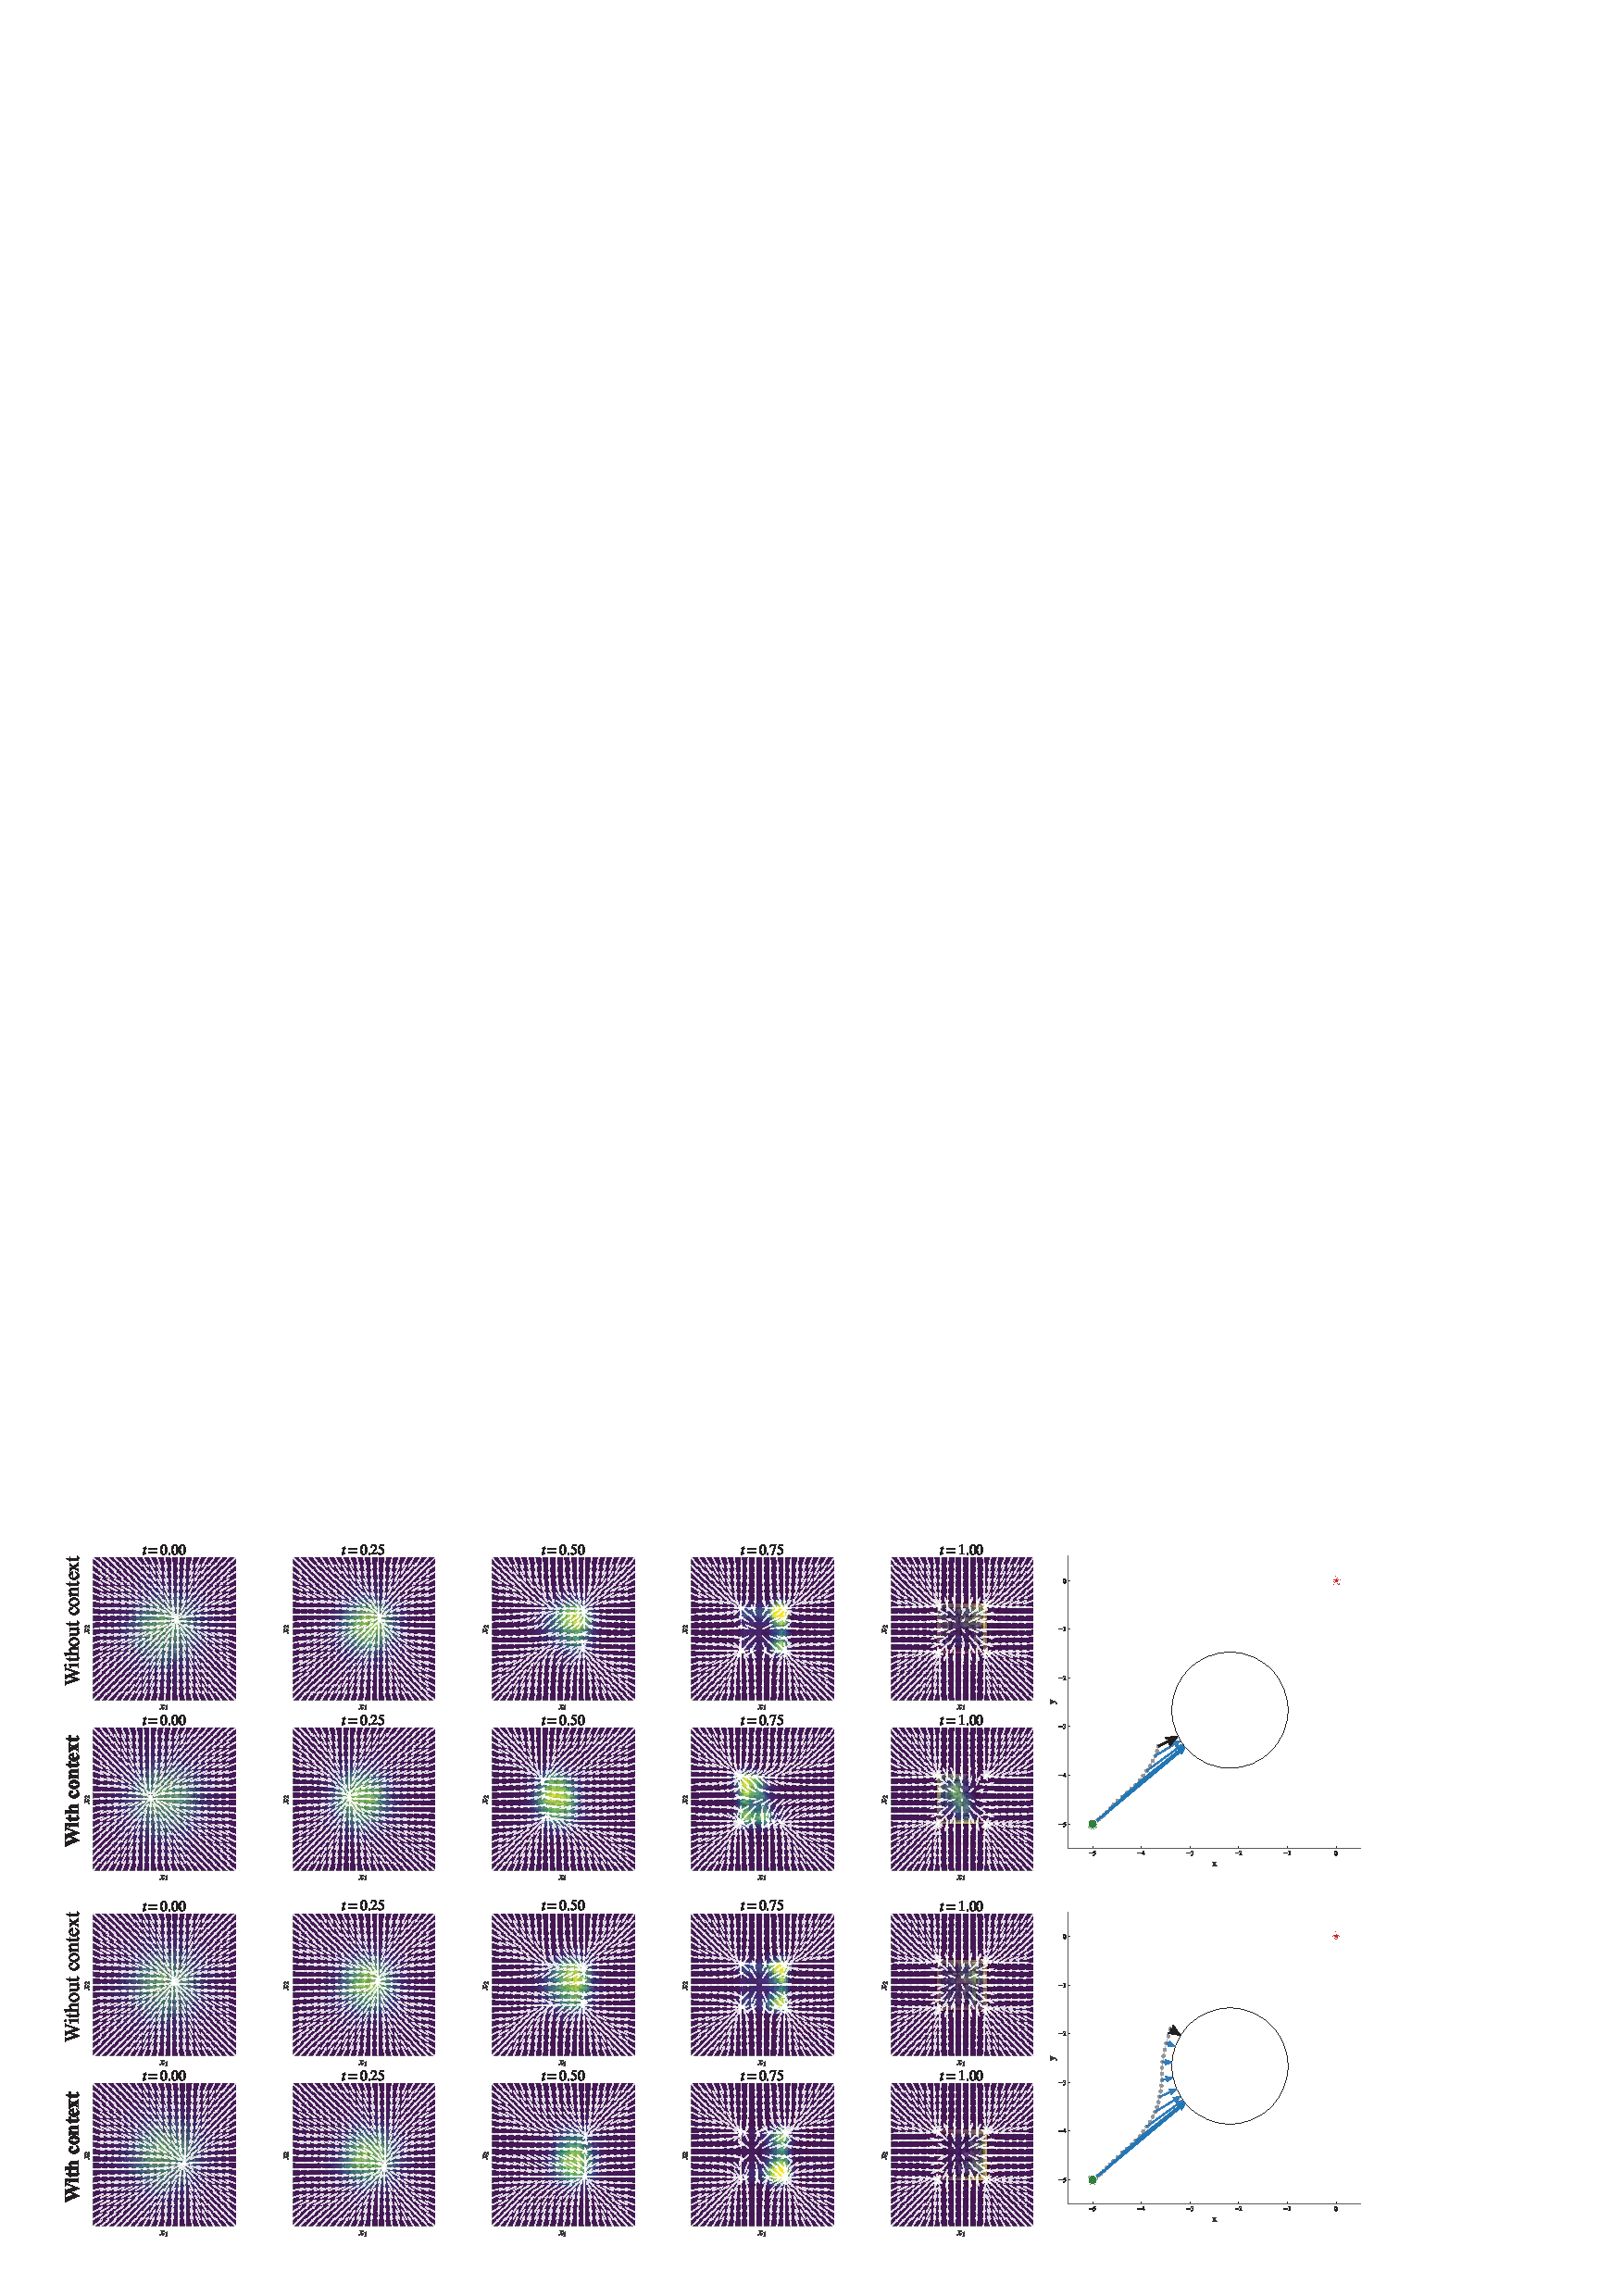
\includegraphics[width=\linewidth]{images/flowmatching_v2.pdf}
%   \caption{
%       Flow matching transforms a simple noise distribution into a target data distribution of safe control policies. \textbf{Without context}, the learned vector field averages all behaviors into a single mode, leading to a greedy, goal-seeking policy (note the concentrated, goal-directed samples at $t=0.75$). \textbf{With context}, the model learns to distinguish between different situations (e.g., passing an obstacle on the left vs. right), enabling it to generate multi-modal, detouring maneuvers.
%     }
%     \vskip -0.4 true in
%   \label{fig:flowmatching}
% \end{figure}

% Before training a policy, we benchmark the performance of our MPPI-DCBF planner against a baseline MPPI controller for the single obstacle case, with results summarized in Table~\ref{tab:mppi_eval}. Both controllers solve the optimal control problem in \eqref{eq:sc-mppi} with identical quadratic cost weights ($Q_p=100I_2, Q_v=10I_2, R=0.05I_2, P_p=1000I_2,$ and $P_v=100I_2$, where the subscripts $p$ and $v$ denote position and velocity, respectively). The baseline MPPI uses an additional penalty-based running cost as in~\eqref{eq:mppisoftconstraint}, $q_{\text{obs}}(x) = 5\cdot10^4 \cdot \mathbf{1}[d_{min}(x)<0] + 100 e^{-d_{min}(x)}$. Analysis of the results reveals several key insights. Most notably, our MPPI-DCBF consistently achieves superior safety guarantees compared to the baseline MPPI method, even at a shorter prediction horizon with lower control cost. Importantly, this comes at a minor computational overhead (2-3 ms per step), indicating that safety is achieved without sacrificing performance.
% % However, we observed that for multi-obstacle cases, (Here say something about multi-obstacle failures)

% \begin{table}[t]
% \caption{MPPI~\cite{williams2017model} and MPPI-DCBF benchmark in terms of computation time, success rate, minimum clearance, and control cost integral. $N$ denotes the prediction horizon for both algorithms.}
% \label{tab:mppi_eval}
% \begin{center}
% \begin{tabular}{|l||c|c|c|c|}
% \hline
% % \multicolumn{5}{|c|}{\textbf{Task: Single obstacle}}\\
% % \hline
% $N=7$ & \shortstack{Comp.\\time [ms]} & \shortstack{Success\\rate [\%]} & \shortstack{Minimum\\distance [m]} & \shortstack{Cost\\Integral} \\
% \hline
% MPPI & 3.6±0.0 & 61.6 & 0.12±0.22 & 1.15±0.29 \\
% \shortstack{MPPI-DCBF\\$(\gamma{=}\,0.1)$} & 5.8±0.0 & 100.0 & 0.65±0.08 & 1.16±0.24 \\
% \shortstack{MPPI-DCBF\\$(\gamma{=}\,0.2)$} & 5.9±0.0  & 100.0 & 0.40±0.11 & 1.10±0.27 \\
% \shortstack{MPPI-DCBF\\$(\gamma{=}\,1.0)$} & 5.8±0.0  & 100.0 & 0.22±0.15 & 1.04±0.27 \\
% \hline
% $N=11$ & \shortstack{Comp.\\time [ms]} & \shortstack{Success\\rate [\%]} & \shortstack{Minimum\\distance [m]} & \shortstack{Cost\\Integral} \\
% \hline
% MPPI & 5.3±0.0 & 100.0 & 0.14±0.09 & 1.91±0.19 \\
% \shortstack{MPPI-DCBF\\$(\gamma{=}\,0.1)$} & 8.9±0.0 & 100.0 & 0.98±0.06 & 1.82±0.11 \\
% \shortstack{MPPI-DCBF\\$(\gamma{=}\,0.2)$} & 8.9±0.0 & 100.0 & 0.66±0.05 & 1.77±0.11 \\
% \shortstack{MPPI-DCBF\\$(\gamma{=}\,1.0)$} & 8.9±0.0 & 100.0 & 0.42±0.06 & 1.77±0.15 \\
% \hline
% \end{tabular}
% \end{center}
% \vskip -0.2 true in
% \end{table}

% We learn these multi-modal behaviors by training the conditional flow matching model, where the bottom row of Fig.~\ref{fig:results_2d} demonstrates that the generative policy successfully reproduces these distinct modalities for different fixed values of $\gamma$. Since the model learns a continuous mapping, it can interpolate between its distinct behaviors seen during training. This enables the synthesis of novel control strategies by implementing a dynamic schedule for $\gamma(k)$ at inference time. Here, we design a heuristic schedule:
% \begin{equation}
% \label{eq:gamma-schedule}
% \gamma(k)=\gamma_{\min}
% +\big(\gamma_{\max}-\gamma_{\min}\big)\,\Big(1-e^{-\beta\, d(k)}\Big)\;e^{-\alpha\,\max\{0,\,v(k)\}}\,,
% \end{equation}
% where $d(k)$ is the distance to the nearest obstacle, $v(k)$ is the relative velocity towards it, and sensitivity parameters $\alpha, \beta$ were fine-tuned to be $0.136, 1.151$, respectively. This schedule is designed to increase conservatism (\textit{i.e.,} lowers $\gamma$) as the robot approaches an obstacle. Fig.~\ref{fig:result_chart} summarizes the performance of the policy over 1000 randomized trials, showing that our adaptive policy achieves a strong balance between safety and feasibility in terms of minimum clearance and success rate. An illustrative example of this behavior in a cluttered environment is shown in Fig.~\ref{fig:result_adaptive}. However, learning an optimal schedule remains an open problem.
% \subsection{Quadrotor}
% \begin{figure}[t]
% \centering
% 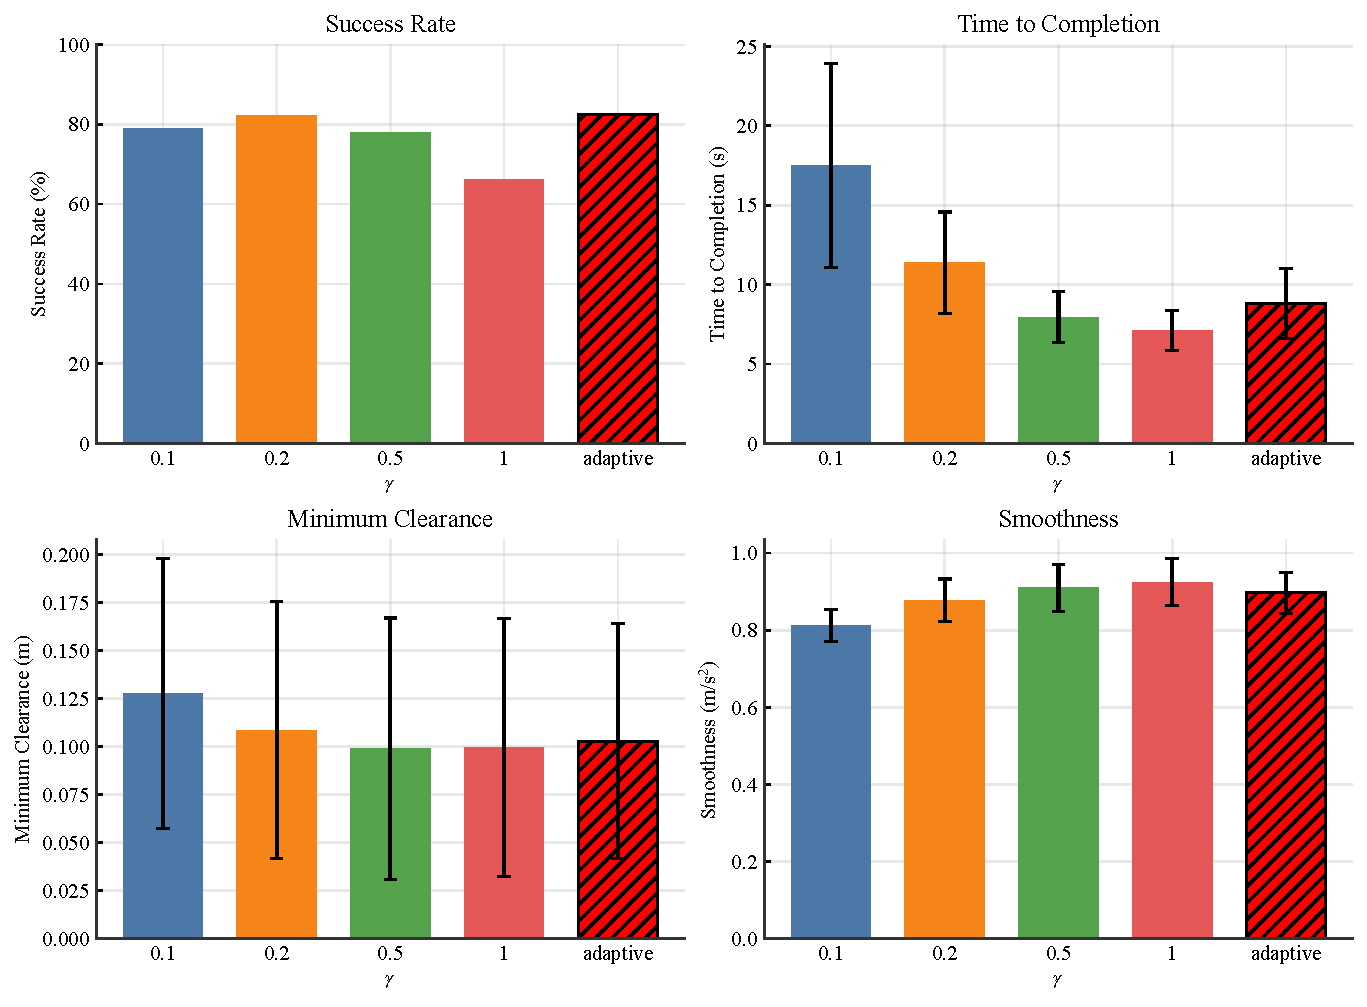
\includegraphics[width=\linewidth]{images/results_chart_v1.pdf}
% \vspace{-.2cm}
% \caption{Performance of the learned generative policy over 1000 randomized trials across four key metrics. The first four bars in each plot correspond to policies using a fixed safety parameter (${\gamma\in\{0.1,0.2,0.5,1.0\}}$). The final hatched bar shows the performance of our adaptive schedule from~\eqref{eq:gamma-schedule}.}
% \label{fig:result_chart}
% \end{figure}

% \begin{figure}[t]
%   \centering
%   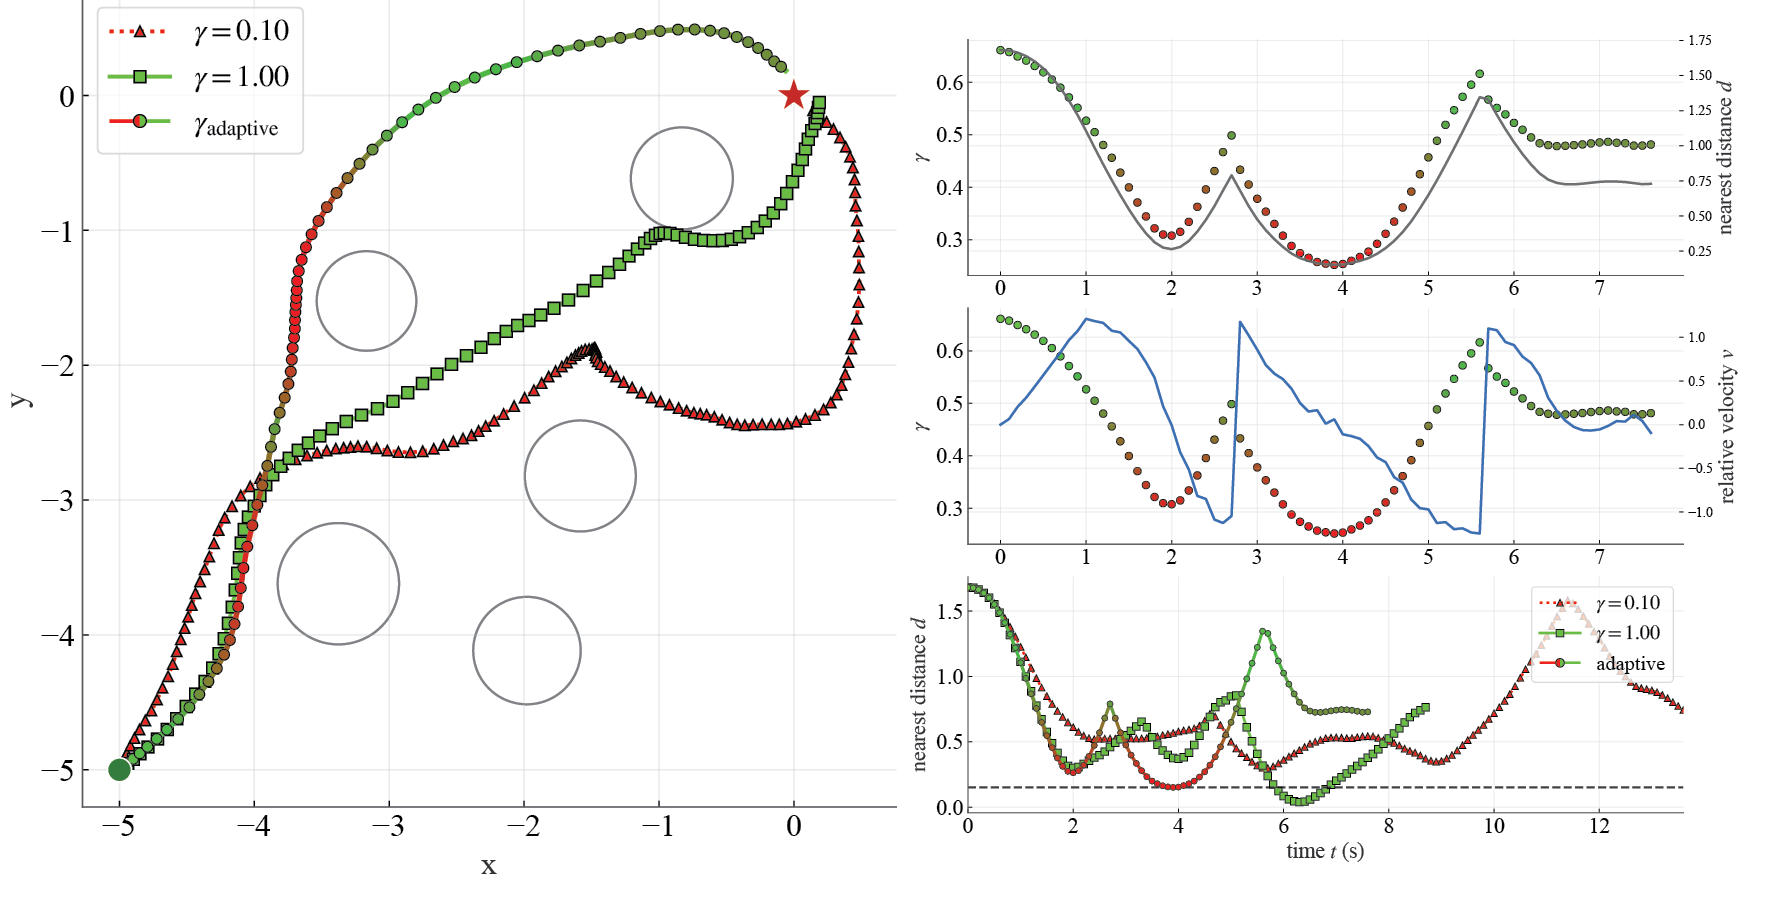
\includegraphics[width=\linewidth]{images/results_adaptive_v2.png}
%   \vspace{-.2cm}
%   \caption{Trajectories generated by the learned generative policy in a single environment under fixed ($\gamma =0.1, 1.0$) and our adaptive $\gamma$ schedule from~\eqref{eq:gamma-schedule}.}
%   \label{fig:result_adaptive}
%   \vskip -0.2 true in
% \end{figure}

% To demonstrate the scalability of our data generation approach to more complex, nonlinear systems, we apply MPPI-DCBF to a simulated quadrotor. The dynamics follow \cite{lee2010geometric}, augmented with second-order motor dynamics:
% % Quadrotor with 2nd-order motor dynamics (compact form)
% \begin{align}
% \frac{d}{dt}\begin{bmatrix}
%     \mathbf{p}\\\mathbf{v}\\ \mathbf{q}\\ \boldsymbol{\omega}\\ \mathbf{w}\\ \dot{\mathbf{w}}\\
% \end{bmatrix}=
% \begin{bmatrix}
% \mathbf{v} \\[0.5mm]
% -\,g\,\mathbf{e}_3 +\frac{1}{m}\,\mathbf R(\mathbf{q})\mathbf{e}_3 \mathbf T(\mathbf{w})\\[0.5mm]
% \tfrac{1}{2}\,\mathbf{q}\otimes(0,\boldsymbol{\omega}) \\[0.5mm]
% -\,\mathbf{J}^{-1}\!\big(\boldsymbol{\omega}\times\mathbf{J}\boldsymbol{\omega}\big)+\mathbf{J}^{-1}\mathbf{M(\mathbf{w})} \\[0.5mm]
% \dot{\mathbf{w}} \\[0.5mm]
% -\tfrac{2\zeta}{\tau}\,\dot{\mathbf{w}} - \tfrac{1}{\tau^{2}}\,\mathbf{w}
% \end{bmatrix}
% +
% \begin{bmatrix}
% \mathbf{0} \\ \mathbf{0} \\ \mathbf{0} \\ \mathbf{0} \\ \mathbf{0} \\ \mathbf{I}_4
% \end{bmatrix}\,\mathbf{u}.
% \label{eq:quad_affine}
% \end{align}
% \noindent where $\mathbf{p}=(x,y,z)\in \mathbb{R}^3$ is the quadrotor's center of mass in the inertial frame, $\mathbf{v}\in\mathbb{R}^3$ is its linear velocity, $\mathbf{q}\in\mathbb{S}^3$ is a quaternion representing body orientation, $\mathbf R(\mathbf{q})\in SO(3)$ is the rotation matrix corresponding to $\mathbf{q}$, $\boldsymbol{\omega}\in\mathbb{R}^3$ is the body angular velocity, $m$ is the total quadrotor mass, $g$ is the gravitational constant, and $\mathbf{J}$ is the matrix of inertia of the body, $\mathbf{e}_3$ is the inertial axis $z$. Motor dynamics are modeled as a second-order system with damping ratio $\zeta$ and time constant $\tau$. With proper scaling, we assume that the input command $\mathbf{u}$ drives the dynamics of the four rotor speeds $\mathbf{w}\in\mathbb{R}^4$. The total thrust $T(\mathbf{w})$, and body moments $\mathbf{M}(\mathbf{w})\in\mathbb{R}^3$, are functions of the resulting rotor speeds.

% Given the high dimensionality and nonlinearity of the system, we employ the one-step predictive safety check mode of our algorithm. In this model, the input command affects the system only through a linear second-order motor model. Since the thrust and moments are evaluated as a function of rotor speed, the discrete dynamics obtained from Euler discretization of the original dynamics are control affine in the current command for a single step. Therefore, the resulting state from the MPPI-DCBF controller remains safe for the next step, as established in Proposition~\ref{prop: 1}. Our planner effectively navigates the quadrotor through a dense field of spherical obstacles, as shown in Fig.~\ref{fig:result_3d}, demonstrating that our core principle can be extended to challenging, nonlinear systems.

% \begin{figure}[t]
%   \centering
%   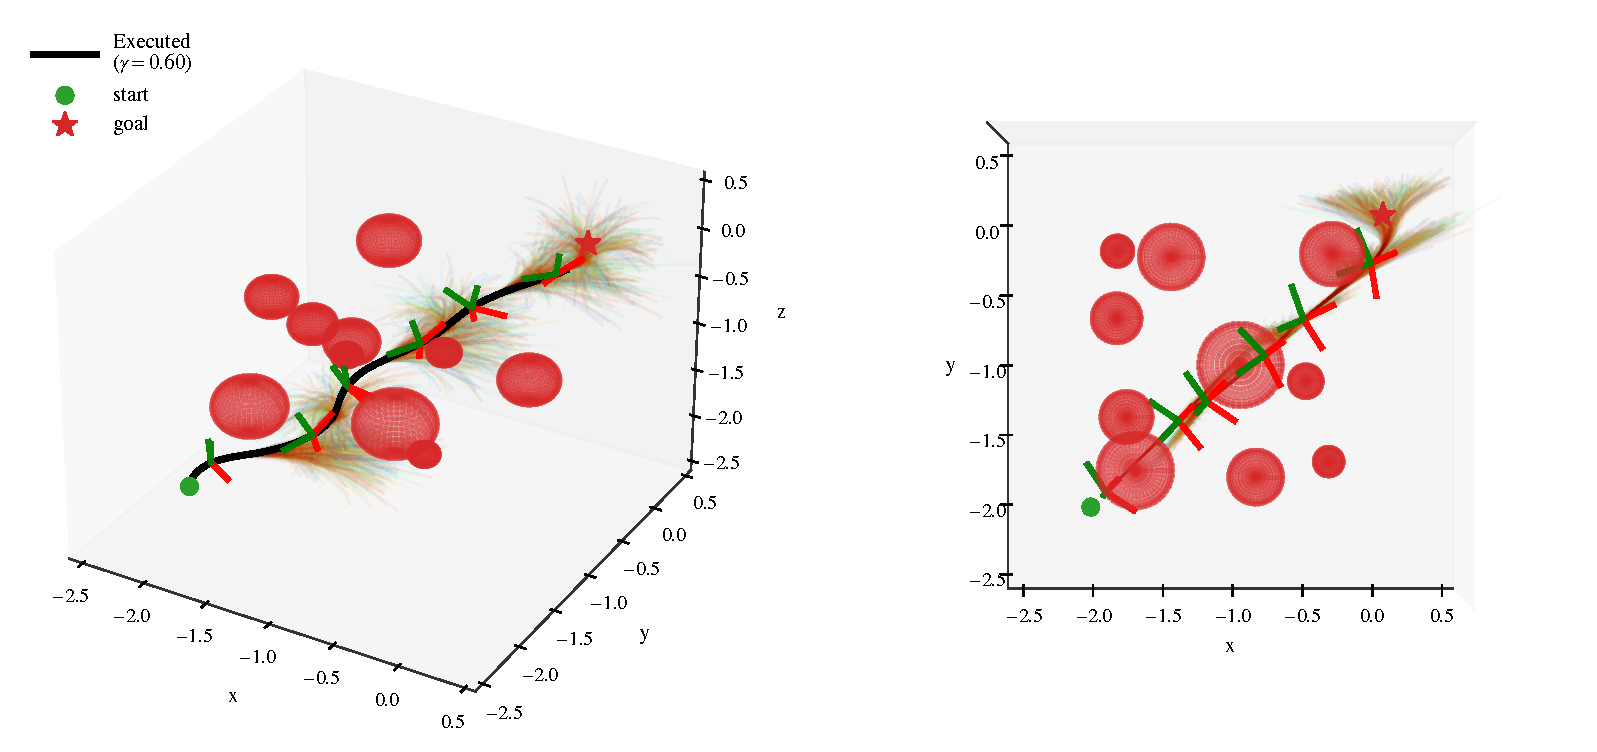
\includegraphics[width=\linewidth]{images/results_3d_v1.pdf}
%   \vspace{-.2cm}
%   \caption{Demonstration of the MPPI-DCBF planner on a quadrotor \eqref{eq:quad_affine} navigating a cluttered 3D environment.}
%   \label{fig:result_3d}
%   \vskip -0.2 true in
% \end{figure}